For example, information about existing power generation capacities is essential for investment planning of conventional and renewable generators \cite{Kendziorski2017,Klein2017}. Detailed information on the geographical location of existing power unit are necessary for power flow optimisation \cite{Amme2018,Mueller2018,Mueller2017}.

Furthermore, different types of times series are a common data input for electricity system models. For example, feed-in time series of solar and wind power as well as load are required for grid simulations or market value analyses \cite{Fusco2017,Tafarte2017,ElAmary2018}. Historic electricity price time series are required for price forecasting \cite{Gonzales2018} and so are load time series for load demand estimations \cite{Yaslan2017}. Moreover, such time series are required for modelling effects of new electricity market designs \cite{Zaidi2018}. 

A combination on both data of existing capacities and historic time series is extensively used in models assessing electricity systems that are in a state of transition or under changing conditions. These include i.a. the system effects of cost reductions of renewables \cite{Gotzens2018}, increased shares of solar self-consumption \cite{Schill2017} or effects on start-up costs of thermal power plants in systems with increasing shares of variable renewables \cite{Schill2017b}. Similar data is required for assessing the need for storage \cite{Zerrahn2018} or the comparison of electricity and hydrogen for transport \cite{Robinius2018}.
Such input data is also essential for analysing the effects of different European climate policy options \cite{Nacken2017}.
For in-depth modelling approaches of wind power feed-in, historic time series are not sufficient and thus detailed meteorological data on wind speed and roughness is additionally required \cite{Olauson2018}.


 %The fact that all references mentioned in Section \ref{subsec:input data requirements} apply data from this platform for their research, shows its relevance for applied energy research.



\item Wolf: hier insbesondere auf laufende Erweiterungen etc. eingehen, möglicherweise auch auf Zielgruppen etc. 
    \item Statistics on how the data is applied, how many users etc., maybe categorize the applications
    \item MaybesShow verification/validation results of bottom-up power plant data with national statisticsja
    \item The approach of OPSD is reproducible, flexible, possible to update and widely apply
    \item quality of the data, room for improvement: what specific?
    \item maintenance work is required
    \item Procedure cannot be applied for all data required for energy system modelling, e.g. for grid stuff probably, there database approaches are also required
    \item tools and knowledge for reproducible data processing and metadata storage is there but data education (documentation, organisation) for energy system modellers and original data owners is a bottleneck while important
    \item legal issue is central, examples of improvement, but data knowledge and knowledge of open licences for original data owners is lacking
    
    
Open electricity system modeling. This report is part of a series of reports on open electricity system modeling. Modeling is running a model (computer code with equations that represent the electricity system) using input data (observed or estimated values) in order to produce output data (results) that can help in answering specific questions (interpretation). This report discusses open input data, i.e. data which is freely accessible and usable, while the next report will focus on open source models, i.e. models for which the computer source code is made public. Broader aspects of open science, such as open access publications, lie outside the scope of these reports.

 

Figure 1. Open data, open source, and open access in relation to the energy modelling process. The focus of this report lies on the first black box: raw data as input to models. Figure updated from Pfenninger et al. (2018) and licensed under CC BY 4.0.
Why open modeling? Open electricity system modelling – using open data in open-source models to produce open results – comes with a range of potential benefits: it can increase the quality of research and policy advice through improved reproducibility and greater scrutiny, increase productivity by allowing reuse and collaborative development, increase credibility and legitimacy in the policy discourse through greater transparency, and makes high-quality data and planning tools accessible to researchers and institutions without the funds for commercial alternatives. Finally, ethical considerations suggest that research financed with public money should be public.
Further readings. Recent articles on open energy system modeling include Pfenninger et al. (2017), Pfenninger et al. (2018) and Morrison (2018).

%To access, subset and download the MERRA-2 database the script uses the OPeNDAP framework which is a standard protocol designed specifically for science data. It provides data types to accommodate meteorological data as well as an interface to access the data. The weather data script translates the user specification to the OPeNDAP interface. After the download of the original data in NetCDF4 format (a three-dimensional data format) the script converts and structures the data before the output parameters are calculated. For example, the original MERRA-2 dataset contains only north and east pointing wind vectors whereas the script uses them to calculate the wind speed. The resulting data can be formatted either in csv or sql-format. Output parameters covered by the script are

Since the total top-of-the-atmosphere and ground horizontal radiation in the original data is not what an energy modeller requires to calculate the resulting energy yield of a solar power plant, the script provides methods to transform these to direct and indirect radiation.

Number of open models increased \cite{openmod2018}
%Why open modeling? Open electricity system modelling – using open data in open-source models to produce open results – comes with a range of potential benefits: it can increase the quality of research and policy advice through improved reproducibility and greater scrutiny, increase productivity by allowing reuse and collaborative development, increase credibility and legitimacy in the policy discourse through greater transparency, and makes high-quality data and planning tools accessible to researchers and institutions without the funds for commercial alternatives. Finally, ethical considerations suggest that research financed with public money should be public.
%Further readings. Recent articles on open energy system modeling include Pfenninger et al. (2017), Pfenninger et al. (2018) and Morrison (2018).

%This is due to the fact, that electricity system models require various input data. 

 Quelle: Open Data. The Benefits -Das volkswirtschaftliche Potential für Deutschland; http://www.kas.de/wf/doc/kas_44906-544-1-30.pdf könnte als Quelle hinsichtlich Kosten etc. vielleicht passen.
 
 Dieser Zustand ändert sich aber gerade immer schneller. Siehe z.B. https://www.govdata.de/ . Würde hier zusätzlich wieder auf einheitliche Standards der zur Dokumentation und Methoden zur Rohdatenbearbeitung nennen oder diese als unter 4. Discussion einbringen .
 
 Vielleicht noch einen Satz zu der deutschen Besonderheit, dass aktuelle eine Doppelte Veröffenlichung stattfindet also TSO's mit netztransparenz.de immer zum Jahresschluss mit 1.5/ 2 Jahren Verzögerung und ab August 2014 die BNetzA auf Ihrer eigenen Seite (monatlich) unterschiedlich veröffentlicht.
 
 
%Output files allow researchers to choose between three different formats: "single index", "multi index" and "stacked". The first two organise the data in tables such that each variable for each country constitutes a separate column, while the time dimension is mapped on the rows. The single index file complies with the Data Package standard in that it contains only one header row, while the multi index format uses the first six rows of a table to describe the data, making it easier to read for humans. The stacked format arranges all variables as one long list (stacking columns on top of each other), which facilitates loading the data in some cases.

% \begin{figure}[!h]
%     \centering
%     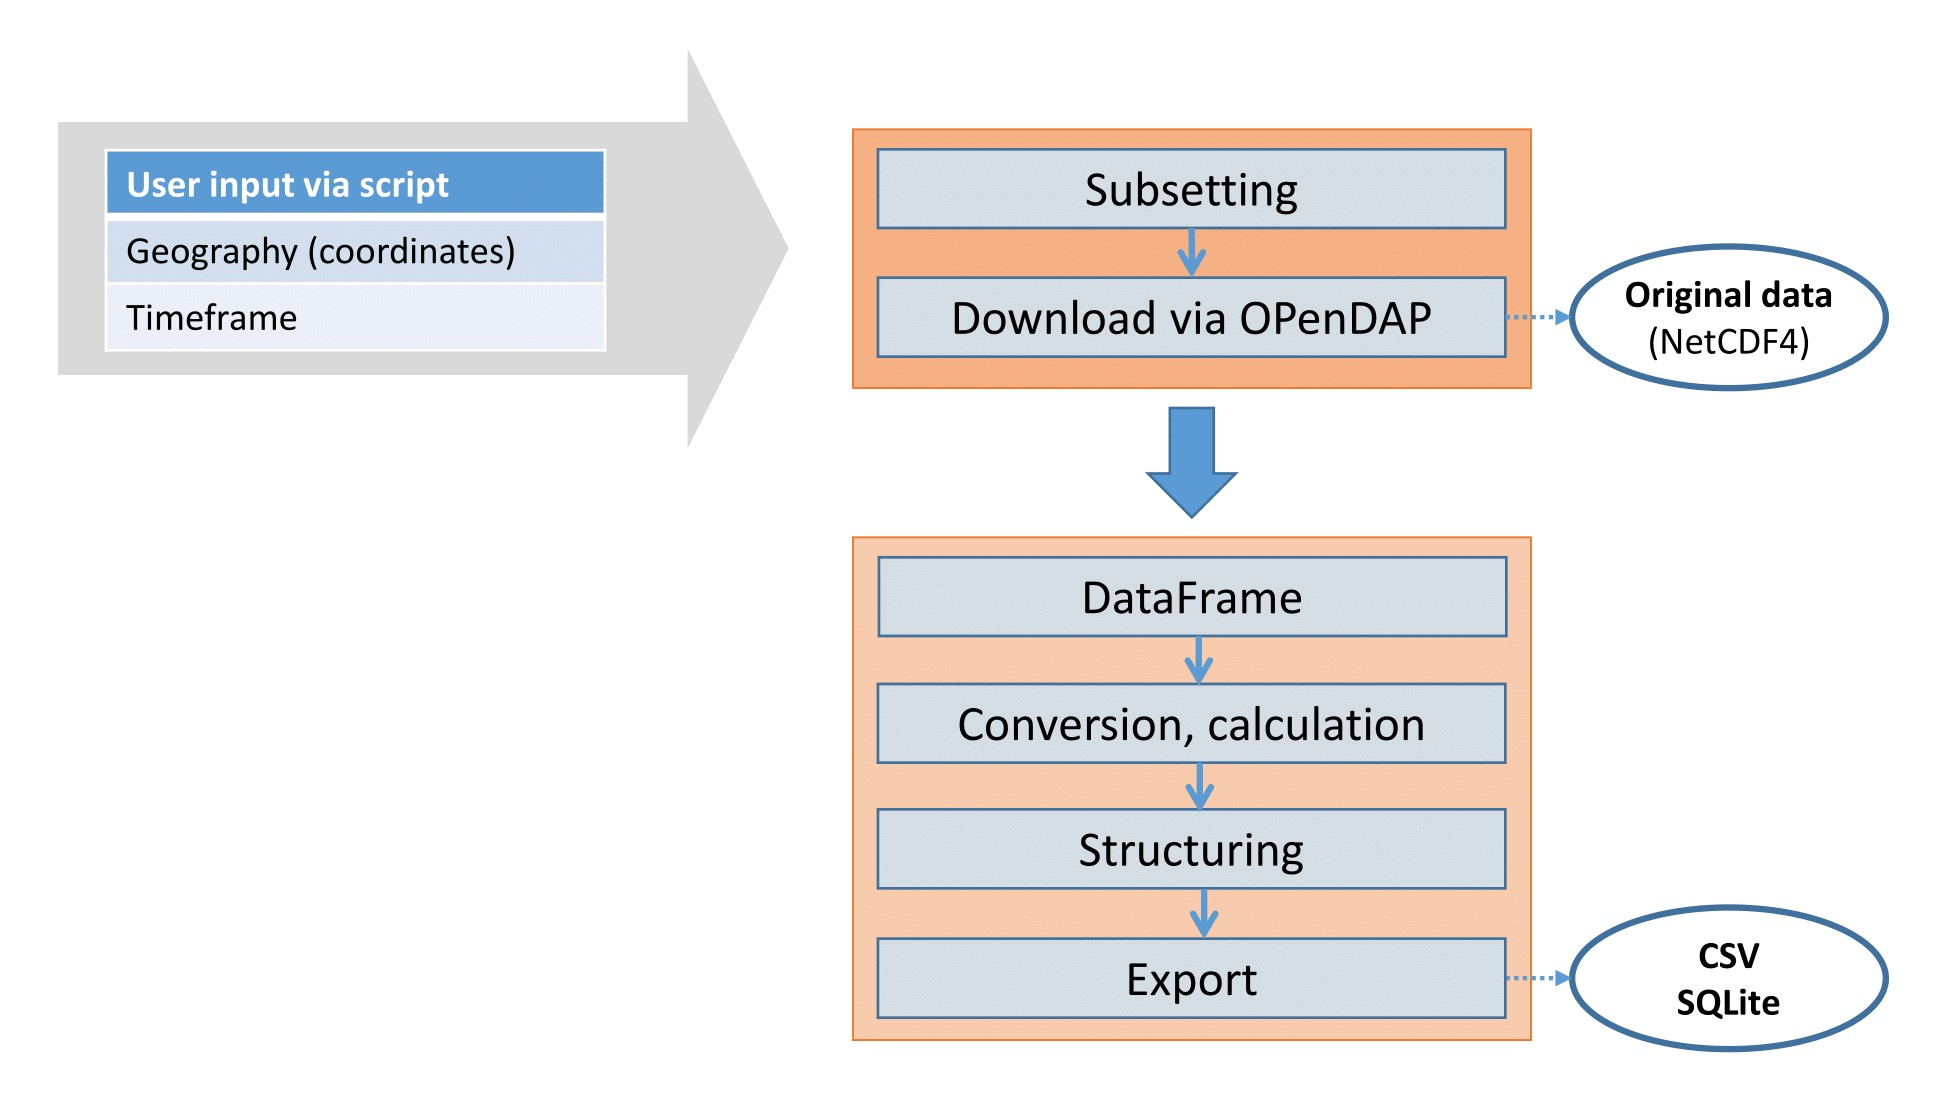
\includegraphics[width=1\textwidth]{figures/weather_data.png}
%     \caption{Content and scope of the weather data script}
%     \label{fig:weather data}
% \end{figure}